\documentclass[12pt]{article}

\usepackage[no-math]{fontspec}
\usepackage{polyglossia}
\setdefaultlanguage[
  indentfirst=true,
  spelling=modern]{russian}
\setotherlanguage{english}

\usepackage{amsmath}
\usepackage{unicode-math}
% \usepackage{booktabs}
% \usepackage{array}
% \usepackage{multirow}

\setmainfont{CMU Serif}
\setsansfont{CMU Sans Serif}
\setmonofont{CMU Typewriter Text}

\setmathfont{Latin Modern Math}

\usepackage{cancel}
% \usepackage{latexsym}
\usepackage{hyperref} % ссылки в документе
\hypersetup{
  colorlinks,
  citecolor=black,
  filecolor=black,
  linkcolor=black,
  urlcolor=black,
  bookmarksdepth=subsubsection, 
  unicode=true,       
  pdftoolbar=true,       
  pdfmenubar=true,    
  pdffitwindow=false,  
  pdfstartview={FitH},  
  pdftitle={Черновик о винтовом движении прямой},
  pdfauthor={Коллектив авторов}
}
\usepackage{graphicx} % картинки
\usepackage{xcolor} % цвет


%~~~~~~~~~~~~~~~~~~~~~~~~~~~~~~~~~~~~~~~~~~~~~~~~~~~~~~~~~~~~~~~~~~~~~~~~~~~~~~~
%								BibLaTeX
%~~~~~~~~~~~~~~~~~~~~~~~~~~~~~~~~~~~~~~~~~~~~~~~~~~~~~~~~~~~~~~~~~~~~~~~~~~~~~~~
\usepackage[autostyle]{csquotes}
\usepackage{url}

\usepackage[%
  backend=biber,
  bibstyle=gost-numeric,
  defernumbers=true,
  movenames=false, % не менять местами заголовок и список авторов, если авторов больше четырех
  maxbibnames=10, % сколько авторов указывать
  sorting=none,
]{biblatex}
% Файл с литературой
\addbibresource{bib/algebra.bib}
\addbibresource{bib/zotero/zotero.bib}



%~~~~~~~~~~~~~~~~~~~~~~~~~~~~~~~~~~~~~~~~~~~~~~~~~~~~~~~~~~~~~~~~~~~~~~~~~~~~~~~
%								Theorems
%~~~~~~~~~~~~~~~~~~~~~~~~~~~~~~~~~~~~~~~~~~~~~~~~~~~~~~~~~~~~~~~~~~~~~~~~~~~~~~~
\usepackage[hyperref,thmmarks]{ntheorem}
\theoremseparator{.}
\theoremsymbol{$\mdlgwhtlozenge$}
\theoremheaderfont{\normalfont\bfseries}
\theorembodyfont{\itshape}
\newtheorem{theo}{Теорема}[section]
\theorembodyfont{\normalfont}
\newtheorem{primer}{Пример}
\theoremstyle{nonumberplain}
\theoremheaderfont{\bfseries}
\newtheorem{dokaz}{Доказательство}
\theoremlisttype{allname}

\author{Подмогильный Иван, Дидусь Кирилл, Геворкян М. Н.}
\date{\today}
\title{Черновик о винтовом движении прямой}

\begin{document}
  
  \maketitle

  \begin{abstract}
    В данном исследовании приводится сравнительный анализ двух подходов к моделированию движения твёрдых тел. Особое внимание уделяется винтовому движению,
      которое является наиболее обобщённой моделью пространственного перемещения твёрдого тела. Анализ литературных источников показал, что представлено
      недостаточное число общедоступных примеров применения винтов в контексте геометрической визуализации, а также наглядных вычислительных примеров использования
        бикватернионов для моделирования трёхмерного движения. Таким образом, проведённое исследование направлено на восполнение пробела в прикладных дидактических
        материалах и методологическую оценку существующих подходов. В работе представлено детальное описание математических формул с пояснениями. Приводятся 
        вычислительные примеры, включая реализацию винтового движения с использованием матричного метода и формулы Родрига.
  \end{abstract}

  %\tableofcontents
  %\clearpage

  % ------------------------------------------------------- Example -------------------------------------------------------
  
  % Книга по алгебре~\cite[Гл. 1 \S 2]{Zulanke:01:2004}. Можно вставить ссылку как сноску, например~\footfullcite{Fedorchuk1990}. Как написано в книге~\fullcite{IlinPosdniak1981}. Ссылка на статью~\cite{PhysRevLett.81.4545} 

  % ------------------------------------------------------- Example -------------------------------------------------------

  \section{Плюккеровы координаты}

  С помощью Плюккеровых координат (также называемых Грассмановыми координатами) \autocite[Гл. 7]{hodgeMethodsAlgebraicGeometry1994}
  можно задать прямую в трёхмерном проективном пространстве $\mathbb{P}^3$ с помощью шести параметров $\mathbf{L}=(\mathbf{v}:\mathbf{m})=(v_1:v_2:v_3:m_1:m_2:m_3)$.
  Где $\mathbf{v}$ называют направляющим вектором прямой, а $\mathbf{m}$ называют моментом прямой. Координаты направляющего вектора и момента можно представить в виде
  Плюккеровой матрицы: 
  \begin{equation*}
    [\mathbf{L}]_\times = 
    \begin{pmatrix}
      0 & -v_1 & -v_2 & -v_3 \\
      v_1 & 0 & -m_1 & -m_2 \\
      v_2 & m_1 & 0 & m_3 \\
      v_3 & m_2 & m_3 & 0
    \end{pmatrix}
  \end{equation*}
  
  \subsection{Движение прямой представленной в Плюккеровых координатах}

  Чтобы подействовать полной линейной группой  GL(3,$\mathbb{R}$) на прямую, можно использовать матрицу преобразования 
  \autocite[Гл. 3.2, секция II. Plücker matrices, пункт 5]{hartley2003multiple}: 

  \begin{equation*}
    \mathbf{H} =
    \begin{pmatrix}
      h_{11} & h_{12} & h_{13} & h_{14} \\
      h_{21} & h_{22} & h_{23} & h_{24} \\
      h_{31} & h_{32} & h_{33} & h_{34} \\
      h_{41} & h_{42} & h_{43} & h_{44} 
  \end{pmatrix}
  \end{equation*}

  Реализацией такого действия будет операция: $[\mathbf{L}']_\times = \mathbf{HLH}^T$.

  \section{Моторы}

  Ещё одним подходом к представлению прямой являются моторы и винты \autocite{dimentberg1965винтовое}. Чтобы определить мотор, нужно задать дуальный вектор
  - $\{\mathbf{v} \mid \mathbf{m}\}$, в котором как и в Плюккеровых координатах $\mathbf{v}$ - направляющий вектор прямой, $\mathbf{m}$ - момент прямой.
  Мотором называется следующая запись: 
  \begin{equation*}
    R = \{ \mathbf{v} \mid \mathbf{m} \} = \mathbf{v} + \varepsilon \mathbf{m}
  \end{equation*}
  Где $\varepsilon$ является дуальным числом $\varepsilon^2=0$. Напомним, что для дуальных чисел выполняется свойство
  \begin{equation*}
    e^{\varepsilon x} = 1 + \varepsilon x
  \end{equation*}

  Изначально дуальные числа были предложены Клиффордом \autocite{cliffordPreliminarySketchBiquaternions1871},
  и в дальнейшем исследованы Штуди \autocite{zindlerGeometrieDynamenStudy1903}.

  \subsection{Винты}

  Для любого мотора можно подобрать такую систему координат, что в ней векторы $\mathbf{v}$ и $\mathbf{m}$ будут коллинеарны. 
  Винтом называется мотор, у которого направляющий вектор и момент коллинеарны $\mathbf{m} \| \mathbf{v}$. Винт имеет запись
  \begin{equation*}
    R = \{ \mathbf{v} \mid p\mathbf{v} \} = \mathbf{v} + \varepsilon p \mathbf{v} = (1+\varepsilon p)\mathbf{v}
  \end{equation*}
  \begin{equation*}
    p=\frac{(\mathbf{v}, \mathbf{m})}{\| \mathbf{v} \|^2}
  \end{equation*}
  В новой системе координат $p$ называется параметром винта.

  Винт, у которого норма направляющего вектора равна единице $\| v \| = 1$ называется единичным винтом. Винт можно записать через единичный винт:
  \begin{equation*}
    R = r(1+\varepsilon p)\mathbf{E} = r e^{\varepsilon p}\mathbf{E}
  \end{equation*}

  \subsection{Движение прямой через винты}
  
  \begin{theo}[Принцип перенесения Котельникова--Штуди]%
  \label{theo:one}  

    Решение любой геометрической или кинематической задачи твёрдого тела с одной неподвижной точкой может использоваться для задачи пространственного движения 
    свободного твёрдого тела.

    Для этого необходимо заменить векторы, вещественные числа, обычные углы и кватернионы на винты, дуальные числа, дуальные углы и бикватернионы соотвественно. 
  \end{theo}

  Согласно принципу перенесения Котельникова-Штуди на прямую в виде винта можно подействовать матрицей поворота в дуальных углах
  
  \begin{equation*}
    R' = \mathcal{R}(A) R, \mathcal{R} \in \mathbb{M}^{3 \times 3}
  \end{equation*}

  Где $A$ - дуальный угол. 

  \subsubsection{Пример}
  Возьмём прямую, лежащую в плоскости $Oxy$ и проходящую через точку $O$ под углом $45^\circ$ к осям $Ox$ и $Oy$. Запишем винт, соответствующий этой прямой.
  Направляющий вектор прямой $\mathbf{v}=(1,1,0)^T$. Произвольная точка прямой - точка $O=(0,0,0)^T$. Если считать, что $\mathbf{v}$ отложен от $O$, то вычислим
  момент по формуле $\mathbf{m} = \mathbf{p} \times \mathbf{v}$ так как $\mathbf{p}=(0,0,0)^T$. Поэтому соответствующий прямой $l$ винт $\mathbf{l}$ можно записать как
  $\mathbf{l} = (1,1,0)^T + \varepsilon (0,0,0)^T = 1 i + 1 j = \mathbf{e}_x + \mathbf{e}_y$.

  Рассмотрим теперь дуальный угол $A=\alpha+\varepsilon \alpha^\circ$ взяв конкретные значения $\alpha=\pi/4$ и $\alpha^\circ=1$. С помощью этого угла повернём прямую $l$
  на угол $\alpha$ против часовой стрелки вокруг оси $Oz$ и поднимем на $1$ вдоль той же оси $Oz$. 

  Чтобы это сделать запишем матрицу для вращения вокруг оси $Oz$ но заменим в ней угол на дуальный.

  \begin{equation*}
    R_z(A)=
    \begin{bmatrix}
      \cos A & -\sin A & 0 \\
      \sin A & \cos A & 0 \\
      0 & 0 & 1
    \end{bmatrix}
  \end{equation*}

  Применим её к винту $\mathbf{l}$.

  \begin{equation*}
    \mathbf{l}'=R_z(A)\mathbf{l}=
    \begin{bmatrix}
      \cos A & -\sin A & 0 \\
      \sin A & \cos A & 0 \\
      0 & 0 & 1
    \end{bmatrix}
    \begin{bmatrix}
      1 \\
      1 \\
      0
    \end{bmatrix}
    =
    \begin{bmatrix}
      \cos A - \sin A \\
      \sin A + \cos A \\
      0
    \end{bmatrix}
  \end{equation*}

  \begin{align*}
      \cos A - \sin A & =\cos \alpha - \varepsilon \alpha^\circ \sin \alpha - \sin \alpha - \varepsilon \alpha^\circ \cos \alpha =
    \cos \alpha - \sin \alpha - (\cos \alpha + \sin \alpha)\varepsilon \alpha^\circ \\
    \cos A + \sin A & = \cos \alpha - \varepsilon \alpha^\circ \sin \alpha + \varepsilon \alpha^\circ \cos \alpha =
    \cos \alpha + \sin \alpha + (\cos \alpha - \sin \alpha)\varepsilon \alpha^\circ
  \end{align*}

  Подставим $A=\pi/4+\varepsilon$ и получим

  \begin{align*}
    \cos A - \sin A & = \cos \pi/4 - \sin \pi/4 + (\cos \pi/4 + \sin \pi/4)\varepsilon = \sqrt{2} \varepsilon \\
    \cos A + \sin A & = \cos \pi/4 + \sin \pi/4 + (\cos \pi/4 - \sin \pi/4)\varepsilon = \sqrt{2}
  \end{align*}

  Из чего следует

  \begin{equation*}
    \mathbf{l}'=
    \begin{bmatrix}
      \sqrt{2} \varepsilon \\
      \sqrt{2} \\
      0
    \end{bmatrix}
    =
    \begin{bmatrix}
      0 \\
      \sqrt{2} \\
      0
    \end{bmatrix}
    + \varepsilon
    \begin{bmatrix}
      \sqrt{2} \\
      0 \\
      0
    \end{bmatrix}
  \end{equation*}

  Если направляющий вектор нормировать то получим:

  \begin{equation*}
    \mathbf{l}' = (0,1,0)^T + \varepsilon (1,0,0)^T
  \end{equation*}

  \section{Бикватернионы}

  Кватернионы могут использоваться для выражения поворотов \autocite[Гл. N]{chelnokov2006кватернионные} так как множество единичных кватернионов 
  \begin{equation*}
    S^3 = \{q \in \mathbb{H} \mid \|q\| =1\}
  \end{equation*}
  по произведению Гамильтона даёт группу Ли, которая дважды покрывает специальную ортогональную группу $SO(3)$ \autocite[Гл. 12]{altmann1986rotations}:
  \begin{equation*}
    \phi : S^3 \rightarrow SO(3), \phi(q) = \phi(-q)
  \end{equation*}

  Бикватернионы получаются из кватернионов процедурой Кейли--Диксона (удвоением) и имеют запись:
  \begin{equation*}
    Q = q + \varepsilon q^o, \quad q,q^o \in \mathbb{H}, \quad \varepsilon^2=0
  \end{equation*}
  Бикватернионы были предложены Клиффордом \autocite{cliffordPreliminarySketchBiquaternions1871}. Более подробно бикватернионы описываются в заметке \autocite{jiaDualQuaternions2018},
  а приложение для свободного движения твёрдого тела (вращение и трансляция) приведено в \autocite[Гл. N]{chelnokov2006кватернионные}

  \subsection{Движение прямой через бикватернионы}

  В алгебре бикватернионов прямая, которую вращают представима в виде чистого бикватерниона
  \begin{equation*}
    \mathbf{L} = L_x i + L_y j + L_z k = \mathbf{v}_\mathbf{L} + \varepsilon \mathbf{m}_\mathbf{L}
  \end{equation*}
  Где $\mathbf{v} = v_x i + v_y j + v_z k$ - направляющий вектор прямой в записи чистого кватерниона и $\mathbf{m} = m_x i + m_y j + m_z k$ - момент прямой в записи чистого кватерниона.
  
  Прямая, которая представляет ось вращения также представима в виде чистого бикватерниона
  \begin{equation*}
    \mathbf{A} = A_x i + A_y j + A_z k = \mathbf{v}_\mathbf{A} + \varepsilon \mathbf{m}_\mathbf{A}
  \end{equation*}

  Движение и поворот прямой задается в виде $\mathbf{L}' = \mathbf{QLQ^*}$. Где бикватернион вращатель записывается в форме
  \begin{equation*}
    \mathbf{Q} = \Lambda_0 + \Lambda_1 i + \Lambda_2 j + \Lambda_3 k
  \end{equation*}
  Его сопряжение 
  \begin{equation*}
    \mathbf{Q}^* = \Lambda_0 - \Lambda_1 i - \Lambda_2 j - \Lambda_3 k
  \end{equation*}
  Лямбда параметры представляют собой
  \begin{equation*}
    \Lambda_0 = \cos{\frac{\Theta}{2}}, \Lambda_1 = \sin{\frac{\Theta}{2}}A_x, \Lambda_2 = \sin{\frac{\Theta}{2}}A_y, \Lambda_3 = \sin{\frac{\Theta}{2}}A_z
  \end{equation*}
  $\Theta$ называется дуальным углом  
  \begin{equation*}
    \Theta  = \theta + \varepsilon \theta^0
  \end{equation*}
  % TODO: (Заметка: переформулировать чтобы объявления были в конце а сначала формулы...)


  % ------------------------------------------------------- Example -------------------------------------------------------
  % Формула может быть в строке $f(x) = \cos{x} + \tg{x} +\ch{x} + \sh{x} + \\sin{x} + e^{-\mathrm{i}x}$ еще формула с дробью $\frac{2}{3}$ и еще $\dfrac{2}{3}$

  % \begin{equation}\label{eq:eq01}
  %   f(x) = \sum\limits^{\infty}_{i=0}\frac{x^2 + 1}{x^3 - 1}
  % \end{equation}

  % В формуле~\eqref{eq:eq01} (сравните \verb|\ref{}|~\ref{eq:eq01})

  % \begin{equation*}
  %   F(x) = \int\limits^{\frac{c-b}{d}}_{a}\dfrac{t^2 - t + 1}{\cos{t}}\mathrm{d} t
  % \end{equation*}

  % \begin{equation*}
  %   \mathbf{v} = \vec{v} = 
  %   \begin{pmatrix}
  %     v^1 \\
  %     v^2 \\
  %     v^3
  %   \end{pmatrix}
  %   \quad
  %   \tilde{u} = 
  %   \begin{bmatrix}
  %     u_1 & u_2 & \ldots & u_n 
  %   \end{bmatrix},
  %   \quad
  %   \mathbf{u} = 
  %   \begin{bmatrix}
  %     u^1\\
  %     \vdots\\
  %     u^n
  %   \end{bmatrix}
  % \end{equation*}

  % \begin{equation*}
  %   M = 
  %   \begin{pmatrix}
  %     a^1_1 & a^1_2 & a^1_3\\
  %     a^2_1 & a^2_2 & a^2_3\\
  %     a^3_1 & a^3_2 & a^3_3
  %   \end{pmatrix}
  %   \quad
  %   a = \mathrm{det}\,A = 
  %   \begin{vmatrix}
  %     a^1_1 & \ldots & a^n_1\\
  %     \vdots & \ddots & \vdots\\
  %     a^1_n & \ldots & a^n_n
  %   \end{vmatrix}
  % \end{equation*}

  % \begin{equation*}
  %   \left\{
  %   \begin{aligned}
  %     &x = y,\\
  %     &x = y + x - 1.
  %   \end{aligned}
  %   \right.
  % \end{equation*}

  % \begin{multline}
  %   x^{15} + x^{15} + x^{15} + x^{15} + x^{15} + x^{15} + x^{15} + x^{15} + x^{15} + x^{15} + x^{15} + x^{15} + x^{15} + x^{15} + {}\\
  %   {} + x^{15} + x^{15} + x^{15} + x^{15} + x^{15} + x^{15} + x^{15} + x^{15} + x^{15} + x^{15} + x^{15} + x^{15} + x^{15} + x^{15} + x^{15} + {} \\
  %   {} + x^{15} + x^{15} + x^{15} + x^{15} + x^{15} + x^{15} + 
  % \end{multline}

  % \begin{gather}
  %   x = y\\
  %   x = p + 3\\
  %   \dfrac{1+5}{5+x}\\
  %   \left\{
  %   \begin{aligned}
  %     &x = y,\\
  %     &x = y + x - 1.
  %   \end{aligned}
  %   \right.
  % \end{gather}

  % \begin{equation*}
  %   \langle x_1, x_2 \rangle, \|\mathbf{v}\|
  %   \quad
  %   a \leqslant 0, \quad a \geqslant 0
  % \end{equation*}

  % \begin{equation*}
  %   x \in \mathbb{R}, \quad \mathbb{C} \ni z
  %   \mathbb{Q} \subset \mathbb{R}
  %   \approx, \between, \not=
  % \end{equation*}

  % \begin{equation}
  %   \alpha \beta \rho \varrho \phi \varphi
  %   \Phi, \Delta, \chi, \varepsilon, \varvarepsilon
  %   \Omega_{\alpha}^{\beta}
  %   \varkappa, \kappa
  %   \quad
  %   \alpha
  % \end{equation}

  % \begin{equation*}
  %   \dot{a},\quad
  %   \ddot{a}, \dddot{a}
  %   \quad
  %   \sqrt{x}, \sqrt[3]{x}
  % \end{equation*}

  % \begin{equation*}
  %   \underbrace{a_1 + b_2}_{=0} + \overbrace{c_2 + x(t)}^{\text{что-то написали}} + a - 1 = 0
  % \end{equation*}


  % \begin{equation*}
  %   \cancel{a_1} + \bcancel{b_2} + \xcancel{c_2} +
  %   \cancelto{0}{x(t)} + a - 1 = 0
  % \end{equation*}

  % \begin{equation}
  %   \mathbf{v}, \vec{v}, \hat{j}, \Vec{j}, \vec{j}
  % \end{equation}

  % \begin{equation*}
  %   \left( \dfrac{\sum^{\infty}_{i=0}{\dfrac{x_i + 1}{x_i - 1}}}{\int\limits^{+\infty}_{-\infty}f(x)\mathrm{d} x} \right)
  % \end{equation*}

  % \begin{equation}
  %   \big( x \Big)
  % \end{equation}


  % \begin{equation*}
  %   \lim_{x \to 0}\dfrac{x^2 + 1}{x^2 - 1}
  % \end{equation*}

  % \begin{equation*}
  %   x^{i\to 0} \Leftrightarrow y^{t \leftarrow 0}
  % \end{equation*}

  % \begin{equation*}
  %   y = \Im{z} \quad x = \Re{z} 
  % \end{equation*}

  % \begin{equation*}
  %   x^{\dag}
  % \end{equation*}

  % \begin{equation*}
  %   \overline{a + b}
  % \end{equation*}

  % \begin{equation*}
  %   C^{k}_{n} = \binom{k}{n}
  % \end{equation*}

  % \begin{equation*}
  %   \tg{x} \quad tg{x}
  %   \\sinh \quad \sh
  % \end{equation*}

  % \begin{equation*}
  %   \mathbb{R}
  %   \quad
  %   R \;\; \mathtt{R}
  %   \quad
  %   \mathcal{R} \quad \mathfrak{R} \mathfrak{G} \mathfrak{S}\mathfrak{L}\mathfrak{K}
  % \end{equation*}

  % Внутри \texttt{абзаца} \(x + 1 = 9\)
  % ------------------------------------------------------- Example -------------------------------------------------------

  \section{Геометрическая алгебра}

  Подробное введение в геометрическую алгебру приводится в книгах [Hitzer, Hestenes D.]. Геометрическая алгебра $\mathbb{G}_{301}$ моделирует трёхмерное проективное
  пространство. Векторами этой алгебры являются элементы $\mathbf{u} = ae_1+be_2+ce_3+\delta e_0 \in \mathbb{G}_{301}$. Можно задать биективное отображение этих векторов
  на перпендикуляры к плоскостям $ax+by+cz+\delta$. Произведение между двумя векторами $\mathbf{u}_1 \mathbf{u}_2$ назывется произведением Клиффорда 
  (или геометрическим произведением). Множество элементов $\mathbb{G}_{301}$ по произведению "сендвича" $\mathbf{u}_1 \mathbf{u}_2 \mathbf{u}_1^{-1}$ образует непрерывную
  группу которую обозначим $G_{Cl}$, эта группа изоморфна группе пинов $G_{Cl} \cong \mathbf{Pin}(p,q,r)$. Произведение сендвича имеет геометрический смысл отражения,
  то есть $\mathbf{u}_1 \mathbf{u}_2 \mathbf{u}_1^{-1}$ интерпретируется как отражение плоскости $\mathbf{u}_2$ относительно плоскости $\mathbf{u}_1$ 
  \autocite{ruheGeometricCliffordAlgebra2023}. 


  \subsection{Движение прямой через геометрическую алгебру}
  Если произвести четыре отражения, то такая операция является винтовым движением. Ниже приводится таблица из статьи 
  \autocite{ruheGeometricCliffordAlgebra2023}. 

  \begin{table}[h!]
    \centering
    \caption{Обзор элементов группы $\mathbf{Pin}(3,0,1)$}
    \label{tab:example}
    \begin{tabular}{|c|c|c|c|} % Use 'c' for centered columns, '|' for vertical lines
    \hline
    \textbf{Кол-во отражений} & \textbf{Элемент группы} & \textbf{Инв-е пр-во} & \textbf{Элемент алгебры} \\ \hline
    % \multicolumn{2}{*}{A} & B1 & C1 & D1 \\ \cline{2-4} % Multirow cell spanning 2 rows
                      %  & B2 & C2 & D2 \\ \hline
    % E1 & \multicolumn{2}{c|}{F1 and G1} & H1 \\ \hline % Multicolumn cell spanning 2 columns
    0 & Единичный эл-т & Объём & Скаляр \\ \hline
    1 & Отражение & Плоскость & Вектор \\ \hline
    2 & Поворот/сдвиг & Прямая & Бивектор \\ \hline
    3 & Рото/трансфлексия & Точка & Тривектор \\ \hline
    4 & Винтовое дв-е & Центр & Четыревектор \\ \hline

    \end{tabular}
  \end{table}

  Приведенное винтовое движение применимо не только к плоскостям, но и к прямым. 


  
  % ------------------------------------------------------- Example -------------------------------------------------------
  % \subsection{Факт №1}

  % A \emph{bulletproof} vest wears Chuck Norris for protection.
  % If Chuck Norris were to travel to an alternate dimension 
  % in which there was another Chuck \emph{Norris} and they both 
  % fought, they would both win. It takes Chuck Norris 
  % 20 minutes        to watch 60 Minutes. Chuck Norris once 
  % shattered the space-time \textbf{continuum}. He felt so bad, 
  % he put it back together. \textit{Chuck Norris} can 
  % sit in the corner of a round room.

  % \subsubsection{Подфакт о Чаке Норрисе}

  % If it looks like chicken, tastes like chicken, and feels like chicken but Chuck Norris says its beef, then it’s beef. Chuck Norris knows Victoria’s secret. Chuck Norris is the reason why Waldo is hiding. When Chuck Norris does a pushup, he’s pushing the Earth down. Chuck Norris invented airplanes because he was tired of being the only person that could fly.

  % Не нумерованный список.
  % \begin{itemize}
  %   \item Пункт номер 1
  %   \item Пункт номер 2
  %   \item Пункт номер 3
  %   на нескольких строках
  %   вполне можно это сделать
  % \end{itemize}

  % Нумерованный список.
  % \begin{enumerate}
  %   \item Пункт номер 1
  %   \item The Great Wall of China was originally created to keep Chuck Norris out. It didn’t work.
  %   \item When Christopher Columbus discovered America, he was greeted by Chuck Norris.
  % \end{enumerate}

  % \begin{description}
  %   \item[№1] Раз
  %   \item[№2] Два
  %   \item[№3] Три Chuck Norris once ordered a steak in a restaurant. The steak did what it was told. Chuck Norris can squeeze orange juice out of a lemon.

  % \end{description}

  % \begin{figure}[h!]
  %   \center
  %   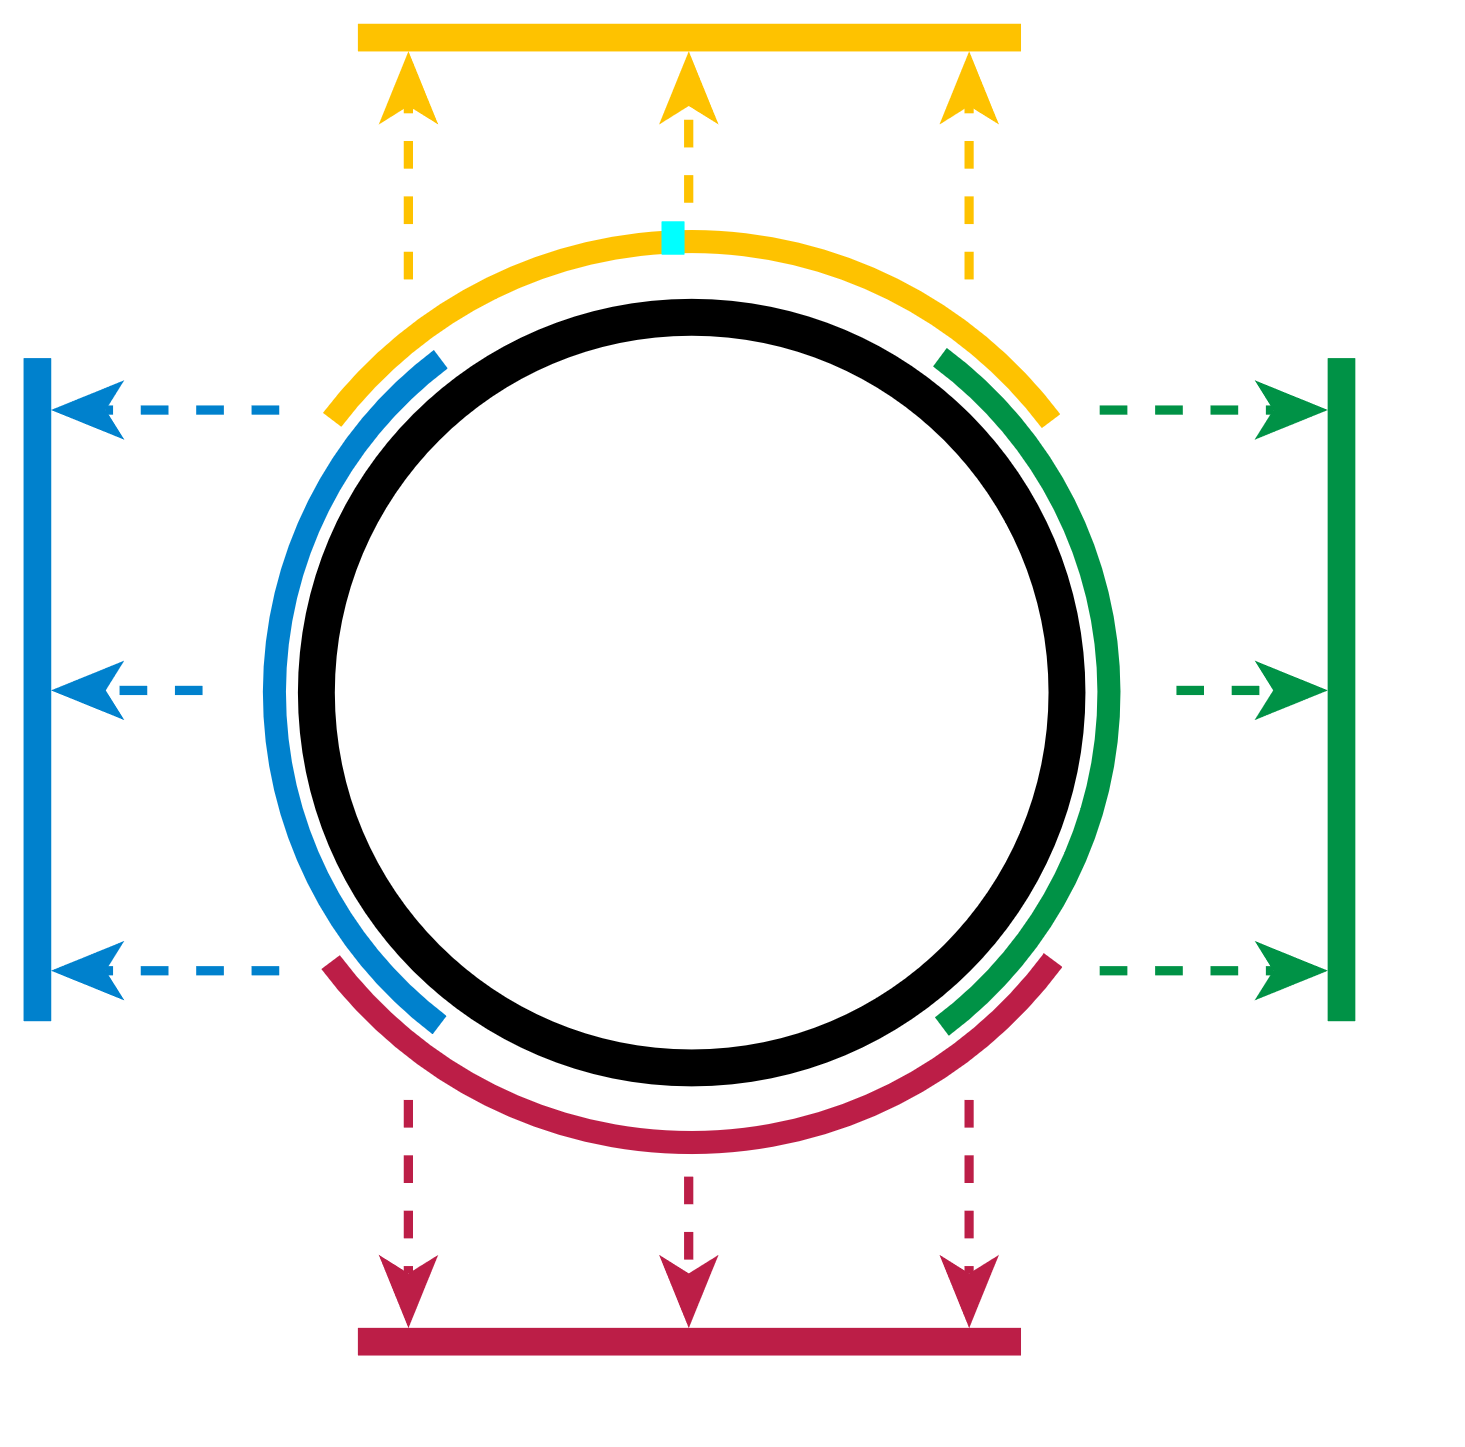
\includegraphics[width=0.5\textwidth]{img/circle.png}
  %   \caption{Подпись к картинке}
  %   \label{fig:img01}
  % \end{figure}

  % Chuck Norris sleeps with a pillow under his gun. Chuck Norris used to beat the shit out of his shadow because it was following to close. It now stands a safe 30 feet behind him. Look at fig.~\ref{fig:img01}. Chuck refers to himself in the fourth person. Chuck Norris once shattered the space-time continuum. He felt so bad, he put it back together. Chuck Norris has never blinked in his entire life. Never.

  

  % \begin{verbatim}
  %   #include <stdio.h>

  %   int main() {
  %     return 0;
  %   }
  % \end{verbatim}

  % Какой-то текст на русском языке.
  % ------------------------------------------------------- Example -------------------------------------------------------

  \printbibliography
  
\end{document}

